\documentclass[a4paper]{article}\usepackage[]{graphicx}\usepackage[]{color}
%% maxwidth is the original width if it is less than linewidth
%% otherwise use linewidth (to make sure the graphics do not exceed the margin)
\makeatletter
\def\maxwidth{ %
  \ifdim\Gin@nat@width>\linewidth
    \linewidth
  \else
    \Gin@nat@width
  \fi
}
\makeatother

\definecolor{fgcolor}{rgb}{0.345, 0.345, 0.345}
\newcommand{\hlnum}[1]{\textcolor[rgb]{0.686,0.059,0.569}{#1}}%
\newcommand{\hlstr}[1]{\textcolor[rgb]{0.192,0.494,0.8}{#1}}%
\newcommand{\hlcom}[1]{\textcolor[rgb]{0.678,0.584,0.686}{\textit{#1}}}%
\newcommand{\hlopt}[1]{\textcolor[rgb]{0,0,0}{#1}}%
\newcommand{\hlstd}[1]{\textcolor[rgb]{0.345,0.345,0.345}{#1}}%
\newcommand{\hlkwa}[1]{\textcolor[rgb]{0.161,0.373,0.58}{\textbf{#1}}}%
\newcommand{\hlkwb}[1]{\textcolor[rgb]{0.69,0.353,0.396}{#1}}%
\newcommand{\hlkwc}[1]{\textcolor[rgb]{0.333,0.667,0.333}{#1}}%
\newcommand{\hlkwd}[1]{\textcolor[rgb]{0.737,0.353,0.396}{\textbf{#1}}}%

\usepackage{framed}
\makeatletter
\newenvironment{kframe}{%
 \def\at@end@of@kframe{}%
 \ifinner\ifhmode%
  \def\at@end@of@kframe{\end{minipage}}%
  \begin{minipage}{\columnwidth}%
 \fi\fi%
 \def\FrameCommand##1{\hskip\@totalleftmargin \hskip-\fboxsep
 \colorbox{shadecolor}{##1}\hskip-\fboxsep
     % There is no \\@totalrightmargin, so:
     \hskip-\linewidth \hskip-\@totalleftmargin \hskip\columnwidth}%
 \MakeFramed {\advance\hsize-\width
   \@totalleftmargin\z@ \linewidth\hsize
   \@setminipage}}%
 {\par\unskip\endMakeFramed%
 \at@end@of@kframe}
\makeatother

\definecolor{shadecolor}{rgb}{.97, .97, .97}
\definecolor{messagecolor}{rgb}{0, 0, 0}
\definecolor{warningcolor}{rgb}{1, 0, 1}
\definecolor{errorcolor}{rgb}{1, 0, 0}
\newenvironment{knitrout}{}{} % an empty environment to be redefined in TeX

\usepackage{alltt}
\usepackage{a4wide}
\usepackage{amsmath, amsfonts, amssymb}
\usepackage{color}
%\usepackage{natbib}

%\addtolength{\textwidth}{1cm}

\newcommand{\tG}{\tilde{G}}
\newcommand{\rmd}{\mathrm{d}}
\newcommand{\rme}{\mathrm{e}}
\newcommand{\rmi}{\mathrm{i}}
\newcommand{\T}{\mathrm{T}}
\newcommand{\nn}{\noindent}
\newcommand{\s}{\boldsymbol{s}}
\newcommand{\bsig}{\boldsymbol{\sigma}}
\newcommand{\z}{\boldsymbol{z}}
\newcommand{\vv}{\boldsymbol{v}}
\newcommand{\be}{\boldsymbol{e}}
\newcommand{\bone}{\boldsymbol{1}}

\newcommand{\eref}[1]{(\ref{#1})}
\IfFileExists{upquote.sty}{\usepackage{upquote}}{}
\begin{document}



\section*{Running a simple MCMC example \hfill \normalsize{\textnormal{Jack Kuipers, \today}}}

\nn For this example we will assume that the score of any DAG is simply proportional to its number of edges.  The size of the DAGs is also restricted to $n=3$

\begin{knitrout}
\definecolor{shadecolor}{rgb}{0.969, 0.969, 0.969}\color{fgcolor}\begin{kframe}
\begin{alltt}
\hlstd{n} \hlkwb{<-} \hlnum{3}
\end{alltt}
\end{kframe}
\end{knitrout}

\nn First we load the \texttt{R} files needed to run the MCMC codes
\begin{knitrout}
\definecolor{shadecolor}{rgb}{0.969, 0.969, 0.969}\color{fgcolor}\begin{kframe}
\begin{alltt}
\hlkwd{source}\hlstd{(}\hlstr{"./edgerevandstructure/structurefns.R"}\hlstd{)}
\hlkwd{source}\hlstd{(}\hlstr{"./edgerevandstructure/structureMCMC.R"}\hlstd{)}
\hlkwd{source}\hlstd{(}\hlstr{"./edgerevandstructure/newedgerevfns.R"}\hlstd{)}
\hlkwd{source}\hlstd{(}\hlstr{"./edgerevandstructure/newedgerevmove.R"}\hlstd{)}
\hlkwd{source}\hlstd{(}\hlstr{"./orderandpartition/orderMCMC.R"}\hlstd{)}
\hlkwd{source}\hlstd{(}\hlstr{"./orderandpartition/orderfns.R"}\hlstd{)}
\hlkwd{source}\hlstd{(}\hlstr{"./orderandpartition/partitionMCMC.R"}\hlstd{)}
\hlkwd{source}\hlstd{(}\hlstr{"./orderandpartition/partitionmoves.R"}\hlstd{)}
\hlkwd{source}\hlstd{(}\hlstr{"./orderandpartition/partitionfns.R"}\hlstd{)}
\hlkwd{source}\hlstd{(}\hlstr{"./orderandpartition/samplefns.R"}\hlstd{)}
\hlkwd{source}\hlstd{(}\hlstr{"./scoring/combinations.R"}\hlstd{)}
\hlkwd{source}\hlstd{(}\hlstr{"./scoring/scorefns.R"}\hlstd{)}
\hlkwd{source}\hlstd{(}\hlstr{"./scoring/scoretables.R"}\hlstd{)}
\hlcom{# load a simple score proportional to the number of edges in}
\hlcom{# the DAG}
\hlkwd{source}\hlstd{(}\hlstr{"./scoring/numedgescore.R"}\hlstd{)}
\end{alltt}
\end{kframe}
\end{knitrout}

\nn Then we build the score table of all parent sets

\begin{knitrout}
\definecolor{shadecolor}{rgb}{0.969, 0.969, 0.969}\color{fgcolor}\begin{kframe}
\begin{alltt}
\hlstd{maxparents} \hlkwb{<-} \hlnum{2}  \hlcom{# Maximum number of parents to allow}
\hlcom{# Fill up a matrix with possible parents}
\hlstd{parenttable} \hlkwb{<-} \hlkwd{listpossibleparents}\hlstd{(maxparents,} \hlkwd{c}\hlstd{(}\hlnum{1}\hlopt{:}\hlstd{n))}
\hlstd{tablelength} \hlkwb{<-} \hlkwd{nrow}\hlstd{(parenttable[[}\hlnum{1}\hlstd{]])}  \hlcom{# size of the table}
\hlcom{# Now need to score them!}
\hlstd{scoretable} \hlkwb{<-} \hlkwd{scorepossibleparents}\hlstd{(parenttable, n)}
\end{alltt}
\end{kframe}
\end{knitrout}

\nn and fix the number of iterations for the various MCMC schemes, recording the outcome at each step

\begin{knitrout}
\definecolor{shadecolor}{rgb}{0.969, 0.969, 0.969}\color{fgcolor}\begin{kframe}
\begin{alltt}
\hlstd{iterations} \hlkwb{<-} \hlnum{100}  \hlcom{# number of iterations in the chain}
\hlstd{stepsave} \hlkwb{<-} \hlnum{1}  \hlcom{# how often to record the DAG}
\end{alltt}
\end{kframe}
\end{knitrout}

\nn We will also perform all the runs with the same seed

\begin{knitrout}
\definecolor{shadecolor}{rgb}{0.969, 0.969, 0.969}\color{fgcolor}\begin{kframe}
\begin{alltt}
\hlstd{seednumber} \hlkwb{<-} \hlnum{101}  \hlcom{# seed number}
\end{alltt}
\end{kframe}
\end{knitrout}

\section{Structure MCMC}

For structure MCMC we include standard edge reversal by setting

\begin{knitrout}
\definecolor{shadecolor}{rgb}{0.969, 0.969, 0.969}\color{fgcolor}\begin{kframe}
\begin{alltt}
\hlstd{revallowed} \hlkwb{<-} \hlnum{1}  \hlcom{# allow standard edge reversals}
\end{alltt}
\end{kframe}
\end{knitrout}
    
\nn and exclude the new edge reversal move by giving the \texttt{moveprobs} vector a single element

\begin{knitrout}
\definecolor{shadecolor}{rgb}{0.969, 0.969, 0.969}\color{fgcolor}\begin{kframe}
\begin{alltt}
\hlstd{moveprobs} \hlkwb{<-} \hlkwd{c}\hlstd{(}\hlnum{1}\hlstd{)}  \hlcom{# having length 1 disallows the new edge reversal move}
\end{alltt}
\end{kframe}
\end{knitrout}

\nn Starting with a DAG with no edges

\begin{knitrout}
\definecolor{shadecolor}{rgb}{0.969, 0.969, 0.969}\color{fgcolor}\begin{kframe}
\begin{alltt}
\hlstd{startDAG} \hlkwb{<-} \hlkwd{matrix}\hlstd{(}\hlkwd{numeric}\hlstd{(n} \hlopt{*} \hlstd{n),} \hlkwc{nrow} \hlstd{= n)}  \hlcom{# starting DAG is empty say}
\end{alltt}
\end{kframe}
\end{knitrout}

\nn we can then run structure MCMC as follows

\begin{knitrout}
\definecolor{shadecolor}{rgb}{0.969, 0.969, 0.969}\color{fgcolor}\begin{kframe}
\begin{alltt}
\hlkwd{set.seed}\hlstd{(seednumber)}  \hlcom{# set the seed}
\hlstd{example} \hlkwb{<-} \hlkwd{structureMCMC}\hlstd{(n, startDAG, iterations, stepsave, maxparents,}
    \hlstd{parenttable, scoretable, revallowed, moveprobs)}  \hlcom{# run the MCMC code}
\end{alltt}
\end{kframe}
\end{knitrout}

\nn The result of the function is a list containing the sampled DAGs (stored as incidence matrices) as the first element and their scores as the second.  We can extract the scores and an example of the DAG with the highest score, represened as its incidence matrix

\begin{knitrout}
\definecolor{shadecolor}{rgb}{0.969, 0.969, 0.969}\color{fgcolor}\begin{kframe}
\begin{alltt}
\hlstd{DAGscores} \hlkwb{<-} \hlkwd{unlist}\hlstd{(example[[}\hlnum{2}\hlstd{]])}
\hlstd{maxscore} \hlkwb{<-} \hlkwd{max}\hlstd{(DAGscores)}
\hlstd{maxDAG} \hlkwb{<-} \hlstd{example[[}\hlnum{1}\hlstd{]][}\hlkwd{which}\hlstd{(DAGscores} \hlopt{==} \hlstd{maxscore)][[}\hlnum{1}\hlstd{]]}
\hlstd{maxDAG}
\end{alltt}
\begin{verbatim}
     [,1] [,2] [,3]
[1,]    0    1    0
[2,]    0    0    0
[3,]    1    1    0
\end{verbatim}
\end{kframe}
\end{knitrout}

\nn The trace plot of the run instead is

\begin{knitrout}
\definecolor{shadecolor}{rgb}{0.969, 0.969, 0.969}\color{fgcolor}\begin{kframe}
\begin{alltt}
\hlstd{nparts} \hlkwb{<-} \hlkwd{length}\hlstd{(example[[}\hlnum{2}\hlstd{]])}
\hlkwd{plot}\hlstd{(}\hlnum{1}\hlopt{:}\hlstd{nparts, DAGscores,} \hlkwc{type} \hlstd{=} \hlstr{"l"}\hlstd{,} \hlkwc{ylab} \hlstd{=} \hlstr{"DAG score"}\hlstd{,} \hlkwc{xlab} \hlstd{=} \hlstr{"iteration step"}\hlstd{,}
    \hlkwc{main} \hlstd{=} \hlstr{""}\hlstd{,} \hlkwc{col} \hlstd{=} \hlstr{"blue"}\hlstd{,} \hlkwc{ylim} \hlstd{=} \hlkwd{c}\hlstd{(maxscore} \hlopt{-} \hlnum{3.2}\hlstd{, maxscore} \hlopt{+}
        \hlnum{0.2}\hlstd{))}
\hlkwd{abline}\hlstd{(}\hlkwc{h} \hlstd{= maxscore,} \hlkwc{col} \hlstd{=} \hlstr{"springgreen4"}\hlstd{,} \hlkwc{lwd} \hlstd{=} \hlnum{3}\hlstd{)}  \hlcom{# the maximal score line}
\hlkwd{lines}\hlstd{(}\hlnum{1}\hlopt{:}\hlstd{nparts, DAGscores,} \hlkwc{type} \hlstd{=} \hlstr{"l"}\hlstd{,} \hlkwc{col} \hlstd{=} \hlstr{"blue"}\hlstd{)}
\end{alltt}
\end{kframe}

{\centering 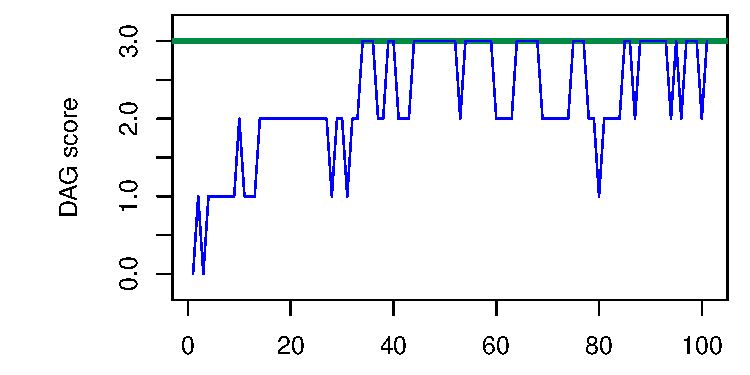
\includegraphics[width=\maxwidth]{figure/minimal-unnamed-chunk-11-1} 

}



\end{knitrout}

\section{New edge reversal move}

We can include the new edge reversal move, by simply making the vector \texttt{moveprobs} have two elements, with the second corresponding to the probability of picking the new edge reversal move.

\begin{knitrout}
\definecolor{shadecolor}{rgb}{0.969, 0.969, 0.969}\color{fgcolor}\begin{kframe}
\begin{alltt}
\hlstd{moveprobs} \hlkwb{<-} \hlkwd{c}\hlstd{(}\hlnum{0.93}\hlstd{,} \hlnum{0.07}\hlstd{)}  \hlcom{# having length 1 disallows the new edge reversal move}
\hlkwd{set.seed}\hlstd{(seednumber)}  \hlcom{# set the seed}
\hlstd{example} \hlkwb{<-} \hlkwd{structureMCMC}\hlstd{(n, startDAG, iterations, stepsave, maxparents,}
    \hlstd{parenttable, scoretable, revallowed, moveprobs)}  \hlcom{# run the MCMC code}
\end{alltt}
\end{kframe}
\end{knitrout}

\nn The trace plot is now

\begin{knitrout}
\definecolor{shadecolor}{rgb}{0.969, 0.969, 0.969}\color{fgcolor}\begin{kframe}
\begin{alltt}
\hlstd{DAGscores} \hlkwb{<-} \hlkwd{unlist}\hlstd{(example[[}\hlnum{2}\hlstd{]])}
\hlstd{maxscore} \hlkwb{<-} \hlkwd{max}\hlstd{(DAGscores)}
\hlstd{nparts} \hlkwb{<-} \hlkwd{length}\hlstd{(example[[}\hlnum{2}\hlstd{]])}
\hlkwd{plot}\hlstd{(}\hlnum{1}\hlopt{:}\hlstd{nparts, DAGscores,} \hlkwc{type} \hlstd{=} \hlstr{"l"}\hlstd{,} \hlkwc{ylab} \hlstd{=} \hlstr{"DAG score"}\hlstd{,} \hlkwc{xlab} \hlstd{=} \hlstr{"iteration step"}\hlstd{,}
    \hlkwc{main} \hlstd{=} \hlstr{""}\hlstd{,} \hlkwc{col} \hlstd{=} \hlstr{"blue"}\hlstd{,} \hlkwc{ylim} \hlstd{=} \hlkwd{c}\hlstd{(maxscore} \hlopt{-} \hlnum{3.2}\hlstd{, maxscore} \hlopt{+}
        \hlnum{0.2}\hlstd{))}
\hlkwd{abline}\hlstd{(}\hlkwc{h} \hlstd{= maxscore,} \hlkwc{col} \hlstd{=} \hlstr{"springgreen4"}\hlstd{,} \hlkwc{lwd} \hlstd{=} \hlnum{3}\hlstd{)}  \hlcom{# the maximal score line}
\hlkwd{lines}\hlstd{(}\hlnum{1}\hlopt{:}\hlstd{nparts, DAGscores,} \hlkwc{type} \hlstd{=} \hlstr{"l"}\hlstd{,} \hlkwc{col} \hlstd{=} \hlstr{"blue"}\hlstd{)}
\end{alltt}
\end{kframe}

{\centering 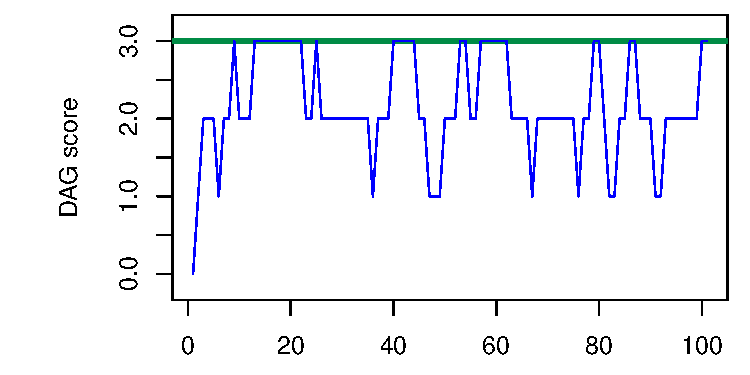
\includegraphics[width=\maxwidth]{figure/minimal-unnamed-chunk-13-1} 

}



\end{knitrout}

\section{Order MCMC}

\nn For Order MCMC we now have three elements in the \texttt{moveprobs} vector.  The first is the probability of swapping any two elements in the order, the second the probability of only swapping adjacent nodes and the last the probability to stay still (to enforce aperiodicity of the chain)

\begin{knitrout}
\definecolor{shadecolor}{rgb}{0.969, 0.969, 0.969}\color{fgcolor}\begin{kframe}
\begin{alltt}
\hlstd{moveprobs} \hlkwb{<-} \hlkwd{c}\hlstd{(}\hlnum{0.99}\hlstd{,} \hlnum{0}\hlstd{,} \hlnum{0.01}\hlstd{)}
\end{alltt}
\end{kframe}
\end{knitrout}

\nn We also need to choose a starting order, for example the identity permutation

\begin{knitrout}
\definecolor{shadecolor}{rgb}{0.969, 0.969, 0.969}\color{fgcolor}\begin{kframe}
\begin{alltt}
\hlstd{startorder} \hlkwb{<-} \hlkwd{c}\hlstd{(}\hlnum{1}\hlopt{:}\hlstd{n)}  \hlcom{# starting order}
\end{alltt}
\end{kframe}
\end{knitrout}

\nn and then we can run the MCMC code

\begin{knitrout}
\definecolor{shadecolor}{rgb}{0.969, 0.969, 0.969}\color{fgcolor}\begin{kframe}
\begin{alltt}
\hlkwd{set.seed}\hlstd{(seednumber)}  \hlcom{# set the seed}
\hlstd{example} \hlkwb{<-} \hlkwd{orderMCMC}\hlstd{(n, startorder, iterations, stepsave, parenttable,}
    \hlstd{scoretable, moveprobs)}
\end{alltt}
\end{kframe}
\end{knitrout}

\nn The output now contains four components, a sampled DAG and its score along with the score of the entire order and the sampled order itself (stored as a permutation vector).  We can again plot the outcome

\begin{knitrout}
\definecolor{shadecolor}{rgb}{0.969, 0.969, 0.969}\color{fgcolor}\begin{kframe}
\begin{alltt}
\hlstd{DAGscores} \hlkwb{<-} \hlkwd{unlist}\hlstd{(example[[}\hlnum{2}\hlstd{]])}
\hlstd{maxscore} \hlkwb{<-} \hlkwd{max}\hlstd{(DAGscores)}
\hlstd{nparts} \hlkwb{<-} \hlkwd{length}\hlstd{(example[[}\hlnum{2}\hlstd{]])}
\hlkwd{plot}\hlstd{(}\hlnum{1}\hlopt{:}\hlstd{nparts, DAGscores,} \hlkwc{type} \hlstd{=} \hlstr{"l"}\hlstd{,} \hlkwc{ylab} \hlstd{=} \hlstr{"DAG score"}\hlstd{,} \hlkwc{xlab} \hlstd{=} \hlstr{"iteration step"}\hlstd{,}
    \hlkwc{main} \hlstd{=} \hlstr{""}\hlstd{,} \hlkwc{col} \hlstd{=} \hlstr{"blue"}\hlstd{,} \hlkwc{ylim} \hlstd{=} \hlkwd{c}\hlstd{(maxscore} \hlopt{-} \hlnum{3.2}\hlstd{, maxscore} \hlopt{+}
        \hlnum{0.2}\hlstd{))}
\hlkwd{abline}\hlstd{(}\hlkwc{h} \hlstd{= maxscore,} \hlkwc{col} \hlstd{=} \hlstr{"springgreen4"}\hlstd{,} \hlkwc{lwd} \hlstd{=} \hlnum{3}\hlstd{)}  \hlcom{# the maximal score line}
\hlkwd{lines}\hlstd{(}\hlnum{1}\hlopt{:}\hlstd{nparts, DAGscores,} \hlkwc{type} \hlstd{=} \hlstr{"l"}\hlstd{,} \hlkwc{col} \hlstd{=} \hlstr{"blue"}\hlstd{)}
\end{alltt}
\end{kframe}

{\centering 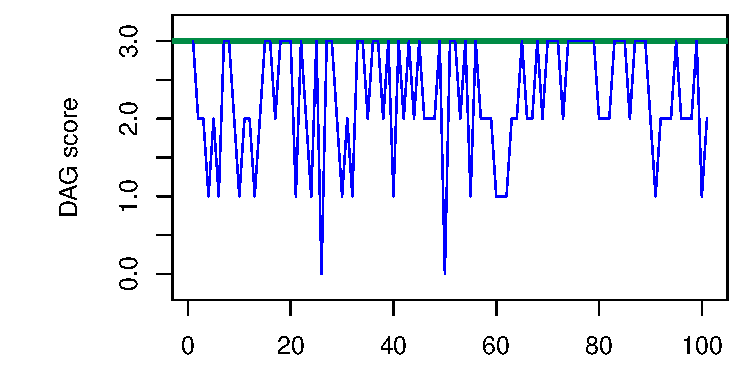
\includegraphics[width=\maxwidth]{figure/minimal-unnamed-chunk-17-1} 

}



\end{knitrout}

\section{Partition MCMC}

\nn For Partiton MCMC we have five elements in the \texttt{moveprobs} vector.  The first is the probability of swapping two nodes from different partititon elements, while the second for swapping nodes from adjacent partition elements.  The third corresponds to joining and splitting partition elements with the fourth being the probability of moving a node from one element to another.  The last is again the probability of not moving

\begin{knitrout}
\definecolor{shadecolor}{rgb}{0.969, 0.969, 0.969}\color{fgcolor}\begin{kframe}
\begin{alltt}
\hlstd{moveprobs} \hlkwb{<-} \hlkwd{c}\hlstd{(}\hlnum{0.4}\hlstd{,} \hlnum{0}\hlstd{,} \hlnum{0}\hlstd{,} \hlnum{0.59}\hlstd{,} \hlnum{0.01}\hlstd{)}
\end{alltt}
\end{kframe}
\end{knitrout}

\nn For the starting partition we can choose the DAG with no edges

\begin{knitrout}
\definecolor{shadecolor}{rgb}{0.969, 0.969, 0.969}\color{fgcolor}\begin{kframe}
\begin{alltt}
\hlstd{startpermutation} \hlkwb{<-} \hlkwd{c}\hlstd{(}\hlnum{1}\hlopt{:}\hlstd{n)}  \hlcom{# pick a starting permutation}
\hlstd{startpartition} \hlkwb{<-} \hlkwd{c}\hlstd{(n)}  \hlcom{# and a starting partition - c(n) gives the empty DAG}
\end{alltt}
\end{kframe}
\end{knitrout}

\nn and then run the MCMC code

\begin{knitrout}
\definecolor{shadecolor}{rgb}{0.969, 0.969, 0.969}\color{fgcolor}\begin{kframe}
\begin{alltt}
\hlkwd{set.seed}\hlstd{(seednumber)}  \hlcom{# set the seed}
\hlstd{example} \hlkwb{<-} \hlkwd{partitionMCMC}\hlstd{(n, startpermutation, startpartition, iterations,}
    \hlstd{stepsave, parenttable, scoretable, moveprobs)}
\end{alltt}
\end{kframe}
\end{knitrout}

\nn The output now contains a five components: a sampled DAG and its score, the score of the entire partition and the sampled permutation and partition.  The trace plot is

\begin{knitrout}
\definecolor{shadecolor}{rgb}{0.969, 0.969, 0.969}\color{fgcolor}\begin{kframe}
\begin{alltt}
\hlstd{DAGscores} \hlkwb{<-} \hlkwd{unlist}\hlstd{(example[[}\hlnum{2}\hlstd{]])}
\hlstd{maxscore} \hlkwb{<-} \hlkwd{max}\hlstd{(DAGscores)}
\hlstd{nparts} \hlkwb{<-} \hlkwd{length}\hlstd{(example[[}\hlnum{2}\hlstd{]])}
\hlkwd{plot}\hlstd{(}\hlnum{1}\hlopt{:}\hlstd{nparts, DAGscores,} \hlkwc{type} \hlstd{=} \hlstr{"l"}\hlstd{,} \hlkwc{ylab} \hlstd{=} \hlstr{"DAG score"}\hlstd{,} \hlkwc{xlab} \hlstd{=} \hlstr{"iteration step"}\hlstd{,}
    \hlkwc{main} \hlstd{=} \hlstr{""}\hlstd{,} \hlkwc{col} \hlstd{=} \hlstr{"blue"}\hlstd{,} \hlkwc{ylim} \hlstd{=} \hlkwd{c}\hlstd{(maxscore} \hlopt{-} \hlnum{3.2}\hlstd{, maxscore} \hlopt{+}
        \hlnum{0.2}\hlstd{))}
\hlkwd{abline}\hlstd{(}\hlkwc{h} \hlstd{= maxscore,} \hlkwc{col} \hlstd{=} \hlstr{"springgreen4"}\hlstd{,} \hlkwc{lwd} \hlstd{=} \hlnum{3}\hlstd{)}  \hlcom{# the maximal score line}
\hlkwd{lines}\hlstd{(}\hlnum{1}\hlopt{:}\hlstd{nparts, DAGscores,} \hlkwc{type} \hlstd{=} \hlstr{"l"}\hlstd{,} \hlkwc{col} \hlstd{=} \hlstr{"blue"}\hlstd{)}
\end{alltt}
\end{kframe}

{\centering 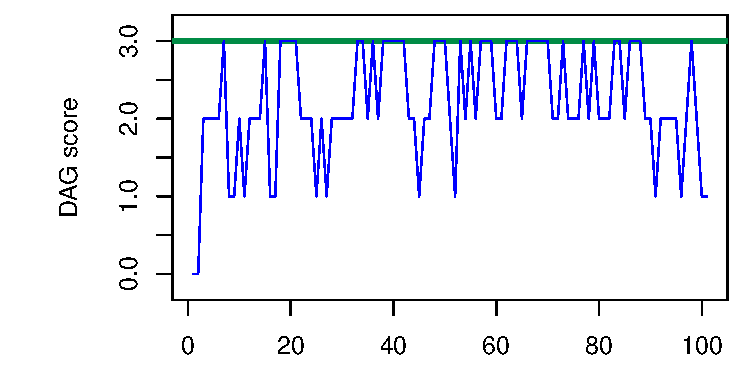
\includegraphics[width=\maxwidth]{figure/minimal-unnamed-chunk-21-1} 

}



\end{knitrout}

\section{Partition MCMC with edge reversal}

\nn Finally we can include the new edge reversal move on an underlying Partition MCMC chain by including a sixth element in the \texttt{moveprobs} vector, corresponding to the probability of picking the edge reversal move

\begin{knitrout}
\definecolor{shadecolor}{rgb}{0.969, 0.969, 0.969}\color{fgcolor}\begin{kframe}
\begin{alltt}
\hlstd{moveprobs} \hlkwb{<-} \hlkwd{c}\hlstd{(}\hlnum{0.37}\hlstd{,} \hlnum{0}\hlstd{,} \hlnum{0}\hlstd{,} \hlnum{0.55}\hlstd{,} \hlnum{0.01}\hlstd{,} \hlnum{0.07}\hlstd{)}
\hlkwd{set.seed}\hlstd{(seednumber)}  \hlcom{# set the seed}
\hlstd{example} \hlkwb{<-} \hlkwd{partitionMCMC}\hlstd{(n, startpermutation, startpartition, iterations,}
    \hlstd{stepsave, parenttable, scoretable, moveprobs)}
\end{alltt}
\end{kframe}
\end{knitrout}

\nn with trace plot

\begin{knitrout}
\definecolor{shadecolor}{rgb}{0.969, 0.969, 0.969}\color{fgcolor}\begin{kframe}
\begin{alltt}
\hlstd{DAGscores} \hlkwb{<-} \hlkwd{unlist}\hlstd{(example[[}\hlnum{2}\hlstd{]])}
\hlstd{maxscore} \hlkwb{<-} \hlkwd{max}\hlstd{(DAGscores)}
\hlstd{nparts} \hlkwb{<-} \hlkwd{length}\hlstd{(example[[}\hlnum{2}\hlstd{]])}
\hlkwd{plot}\hlstd{(}\hlnum{1}\hlopt{:}\hlstd{nparts, DAGscores,} \hlkwc{type} \hlstd{=} \hlstr{"l"}\hlstd{,} \hlkwc{ylab} \hlstd{=} \hlstr{"DAG score"}\hlstd{,} \hlkwc{xlab} \hlstd{=} \hlstr{"iteration step"}\hlstd{,}
    \hlkwc{main} \hlstd{=} \hlstr{""}\hlstd{,} \hlkwc{col} \hlstd{=} \hlstr{"blue"}\hlstd{,} \hlkwc{ylim} \hlstd{=} \hlkwd{c}\hlstd{(maxscore} \hlopt{-} \hlnum{3.2}\hlstd{, maxscore} \hlopt{+}
        \hlnum{0.2}\hlstd{))}
\hlkwd{abline}\hlstd{(}\hlkwc{h} \hlstd{= maxscore,} \hlkwc{col} \hlstd{=} \hlstr{"springgreen4"}\hlstd{,} \hlkwc{lwd} \hlstd{=} \hlnum{3}\hlstd{)}  \hlcom{# the maximal score line}
\hlkwd{lines}\hlstd{(}\hlnum{1}\hlopt{:}\hlstd{nparts, DAGscores,} \hlkwc{type} \hlstd{=} \hlstr{"l"}\hlstd{,} \hlkwc{col} \hlstd{=} \hlstr{"blue"}\hlstd{)}
\end{alltt}
\end{kframe}

{\centering 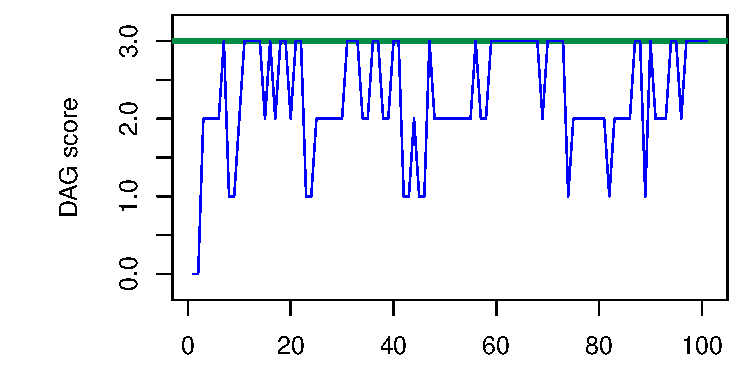
\includegraphics[width=\maxwidth]{figure/minimal-unnamed-chunk-23-1} 

}



\end{knitrout}

\end{document}
